\chapter{Noticias relativas a: Ataques de ransomware contra corporaciones y gobiernos}


    \section{Breve descripción de la amenaza: (más de 100 palabras)}
    
    La amenaza descrita consiste en un ataque de ransomware de doble extorsión ejecutado por el grupo criminal ``Interlock''. 
    Esta modalidad de ataque no solo se limita al cifrado de archivos críticos para paralizar las operaciones de la entidad víctima 
    (en este caso, un ``proveedor'' de servicios de diálisis), sino que incluye la exfiltración previa de volúmenes masivos 
    de datos sensibles. El grupo Interlock utilizó técnicas avanzadas para infiltrarse en la red de DaVita, logrando permanecer
     de forma persistente desde el 24 de marzo hasta el 12 de abril de 2025. Durante este periodo, los atacantes extrajeron 
     aproximadamente 20 terabytes de información, incluyendo bases de datos SQL con más de 200 millones de registros. 
     El ransomware afectó principalmente a los servidores de laboratorio y bases de datos clínicas. Al no concretarse el 
     pago del rescate, los atacantes procedieron a la filtración selectiva de los datos en su sitio de la ``Dark Web'', utilizando
      la exposición de información de salud protegida (PHI) como mecanismo de presión.

    \section{Fecha de la noticia:}
    22 de agosto de 2025

    \section{Título de la noticia:}
    \href{https://www.hipaajournal.com/davita-ransomware-attack/}{DaVita Confirms 2.7 Million Individuals Affected by Ransomware Attack}

    % 2. Enlaces y Medio
    \section{Enlace a la noticia:}

    \href{https://www.hipaajournal.com/davita-ransomware-attack/}{https://www.hipaajournal.com/davita-ransomware-attack/}

    \section{Medio:}
    The HIPAA Journal
    
    \section{Enlace al medio:}
    \href{https://www.hipaajournal.com/}{https://www.hipaajournal.com/}

    \section{Nacionalidad del medio:}
    Estados Unidos
    
    \section{Idioma de la noticia:}
    Inglés
    
    \section{Pequeña imagen de la noticia:}
    \vspace{1em}
    \begin{center}
        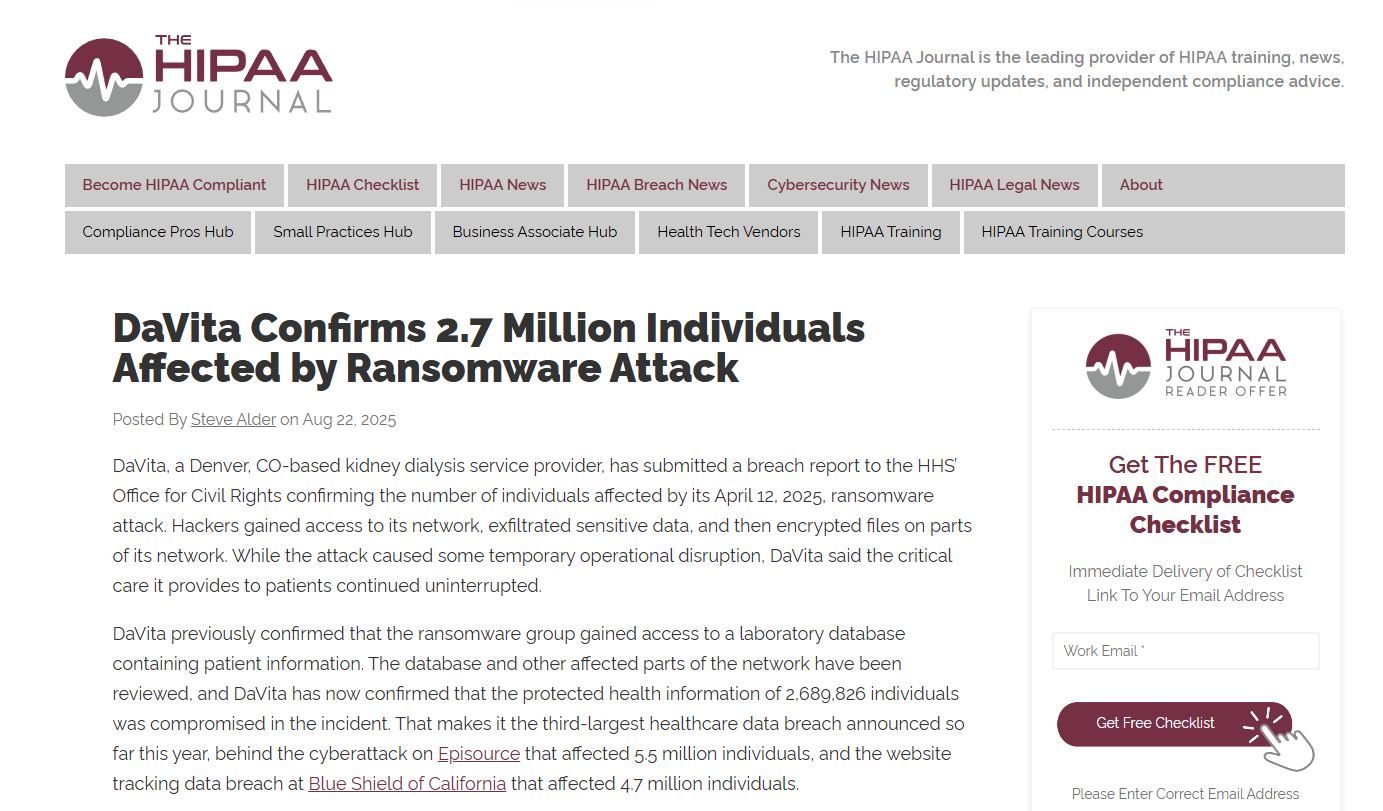
\includegraphics[width=0.8\textwidth]{Imagenes/04-ran.png} 
    \end{center} 

    % 4. Resumen y Análisis
    \section{Breve resumen de la noticia: (más de 100 palabras)}
    DaVita, uno de los mayores proveedores de servicios de diálisis en EE. UU., confirmó que un ataque de ransomware ocurrido en 
    abril de 2025 afectó finalmente a 2.689.826 personas. El incidente, atribuido al grupo Interlock, supuso el acceso no autorizado 
    a servidores de red y bases de datos de laboratorio. Aunque la empresa logró mantener la continuidad del tratamiento 
    crítico para sus pacientes, la brecha de seguridad resultó en la exfiltración de 20 TB de datos sensibles, incluyendo nombres, números de Seguro Social, información de seguros médicos y resultados de pruebas de laboratorio. El informe financiero de la compañía reveló que el ataque generó costes de remediación de 13,5 millones de dólares solo en el segundo trimestre de 2025. Tras el fracaso de las negociaciones de rescate, el grupo atacante comenzó a publicar archivos robados en su portal de filtraciones. Como respuesta, DaVita ha comenzado a enviar cartas de notificación a los afectados, ofreciendo servicios de monitoreo de crédito y protección de identidad, mientras enfrenta al menos dos demandas colectivas por presunta negligencia en la custodia de los datos.

    \section{Relación con la amenaza:}
    La noticia es un ejemplo crítico de ataque de ransomware contra una infraestructura corporativa de salud. Ilustra cómo las corporaciones que manejan datos sensibles son objetivos prioritarios debido al alto valor de la información médica y la presión operativa para restaurar servicios vitales.

    \section{\textquestiondown Existe CVE o CWE asociado a la noticia?}
    La noticia no menciona un código CVE específico.

    \section{Impacto ocasionado por la amenaza en esta noticia: (más de 100 palabras)}
    El impacto de este ataque es masivo y se divide en tres vertientes: financiera, operativa y legal. 
    Financieramente, DaVita reportó pérdidas directas de 13,5 millones de dólares destinados a especialistas en ciberseguridad, 
    restauración de sistemas y costes administrativos, sin contar las pérdidas potenciales por interrupción de negocio y multas. 
    Operativamente, aunque la atención al paciente no se detuvo, hubo una interrupción significativa 
    en los procesos de laboratorio y administrativos que obligó a implementar procesos manuales temporales. 
    Desde el punto de vista legal y reputacional, la filtración de datos de 2,7 millones de personas ha derivado en demandas 
    colectivas (como \textit{Reid v. Davita Inc.}) y una investigación de la Oficina de Derechos Civiles (OCR). 
    La exposición de números de Seguro Social y datos clínicos coloca a los pacientes en un riesgo prolongado de robo de 
    identidad y fraude médico, lo que erosiona profundamente la confianza en la institución y requiere inversiones a 
    largo plazo en servicios de protección para los afectados.

